\section{An initial overview of of the course}
\title[Initial overview]{Power Electronics Devices and Components}
 
\begin{frame}[plain]
    \titlepage
\end{frame}
%%%%%%%%%%%%%%%%%%%%%%%%%%%%%%%%%%%%%%%%%%%%%%%%%%%%%%%%%%%%%
%% Overview of the course %%
%%%%%%%%%%%%%%%%%%%%%%%%%%%%%%%%%%%%%%%%%%%%%%%%%%%%%%%%%%%%%
\begin{frame}
	\frametitle{Course Overview}
The course will be in 6 modules.
		\begin{itemize}
		  \item Module I: Introduction to Automation Technologies.
		  \item Module II: Sensor Technologies.
		  \item Module III: Signal Conditioning.
		  \item Module IV: Processors in Automation Systems.
		  \item Module V: Controllers and Communication.
%		  \item Module VI: Industrial communication systems.
		  \item Module VI: Actuators and Motion Systems.
		  \item Module VII: Testing and Validation.
		  \item Module VIII: Industrial Case Studies.
		\end{itemize}
\textbf{Pattern of class}: \\ Day: Tuesday, every week \\ 
Time: 8 am to 10 am (theory) and 10 am to 12 am (tutorial) (ideally but it can change) \\
Holidays: 23 Dec 2025, 30 Dec 2025, and 6 Jan 2026. %As required classes will be rescheduled. 
\end{frame}

%%%%%%%%%%%%%%%%%%%%%%%%%%%%%%%%%%%%%%%%%%%%%%%%%%%%%%%%%%%%%
%% Teaching Support Team %%
%%%%%%%%%%%%%%%%%%%%%%%%%%%%%%%%%%%%%%%%%%%%%%%%%%%%%%%%%%%%%
\begin{frame}
	\frametitle{The teaching team}
	\vspace{-0.5cm}
	\begin{columns}[t]
\centering
		\column[T]{0.33\textwidth}
		\begin{figure}
			\centering
				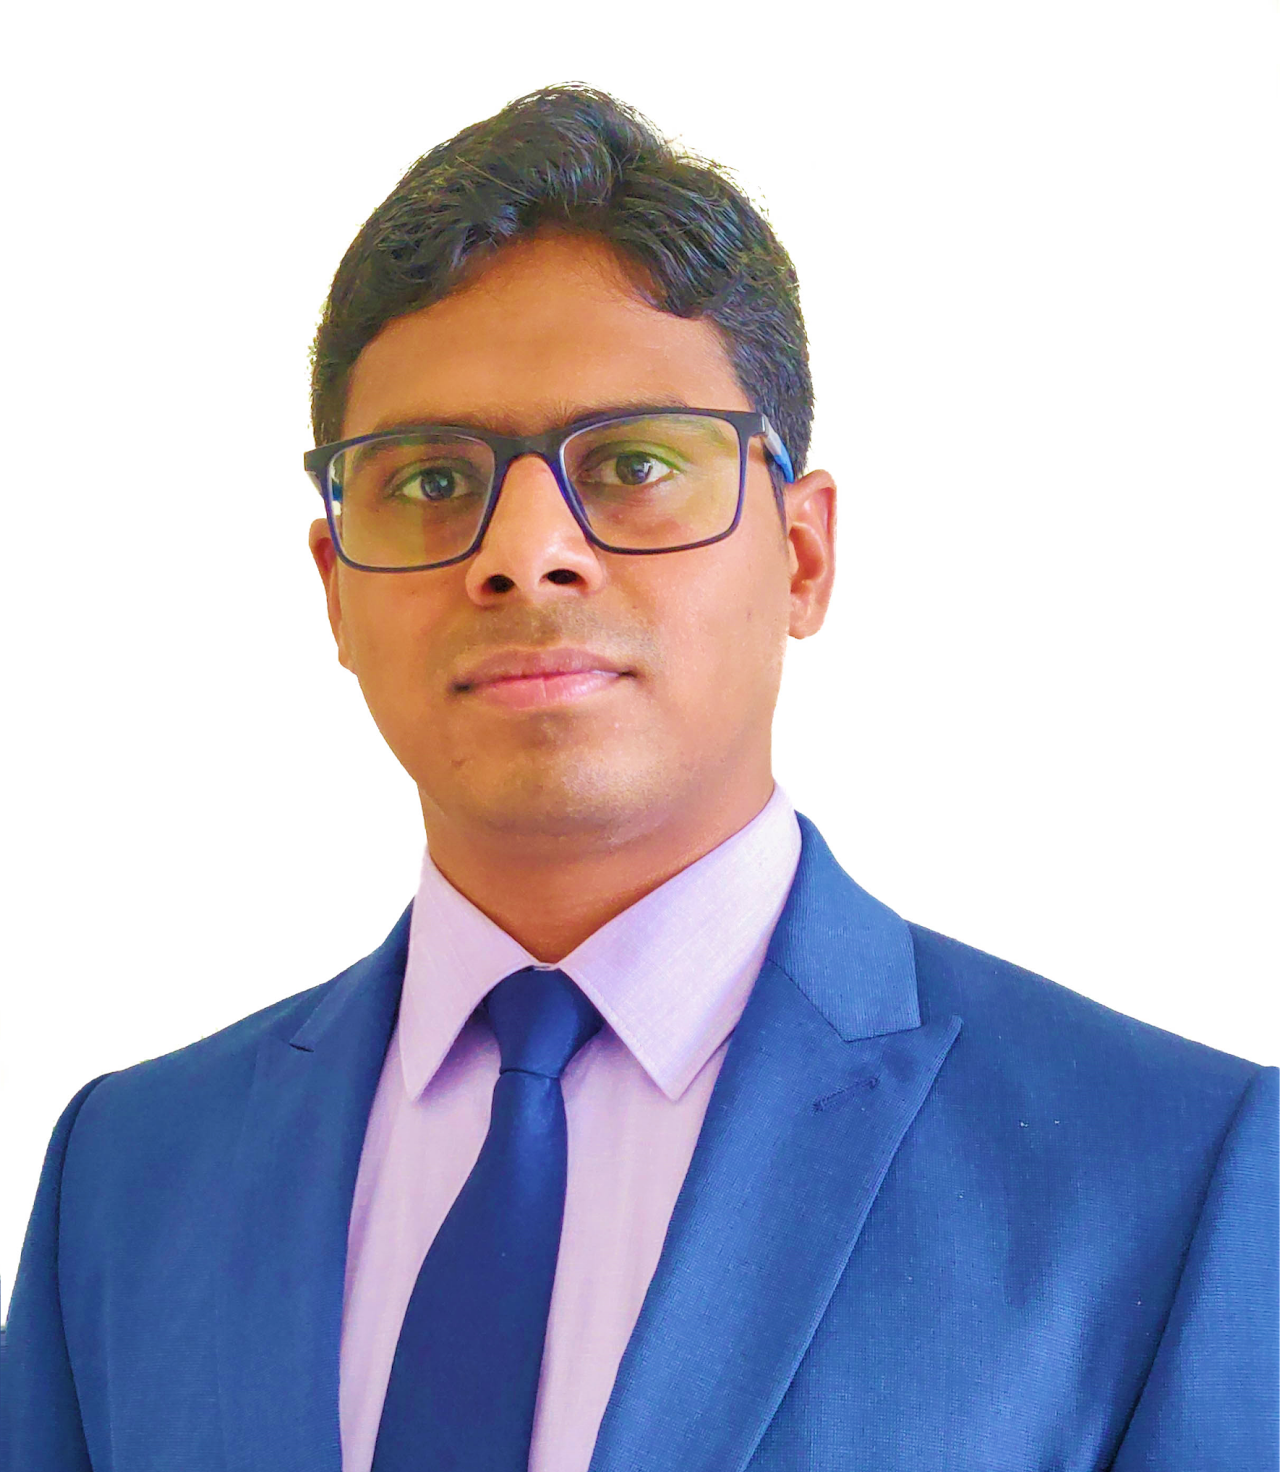
\includegraphics[height=2.5cm]{fig/lec01/Bikash.png}
				\caption*{Bikash Sah}
		\end{figure}
	
		\column[T]{0.33\textwidth}
		\begin{figure}
			\centering
				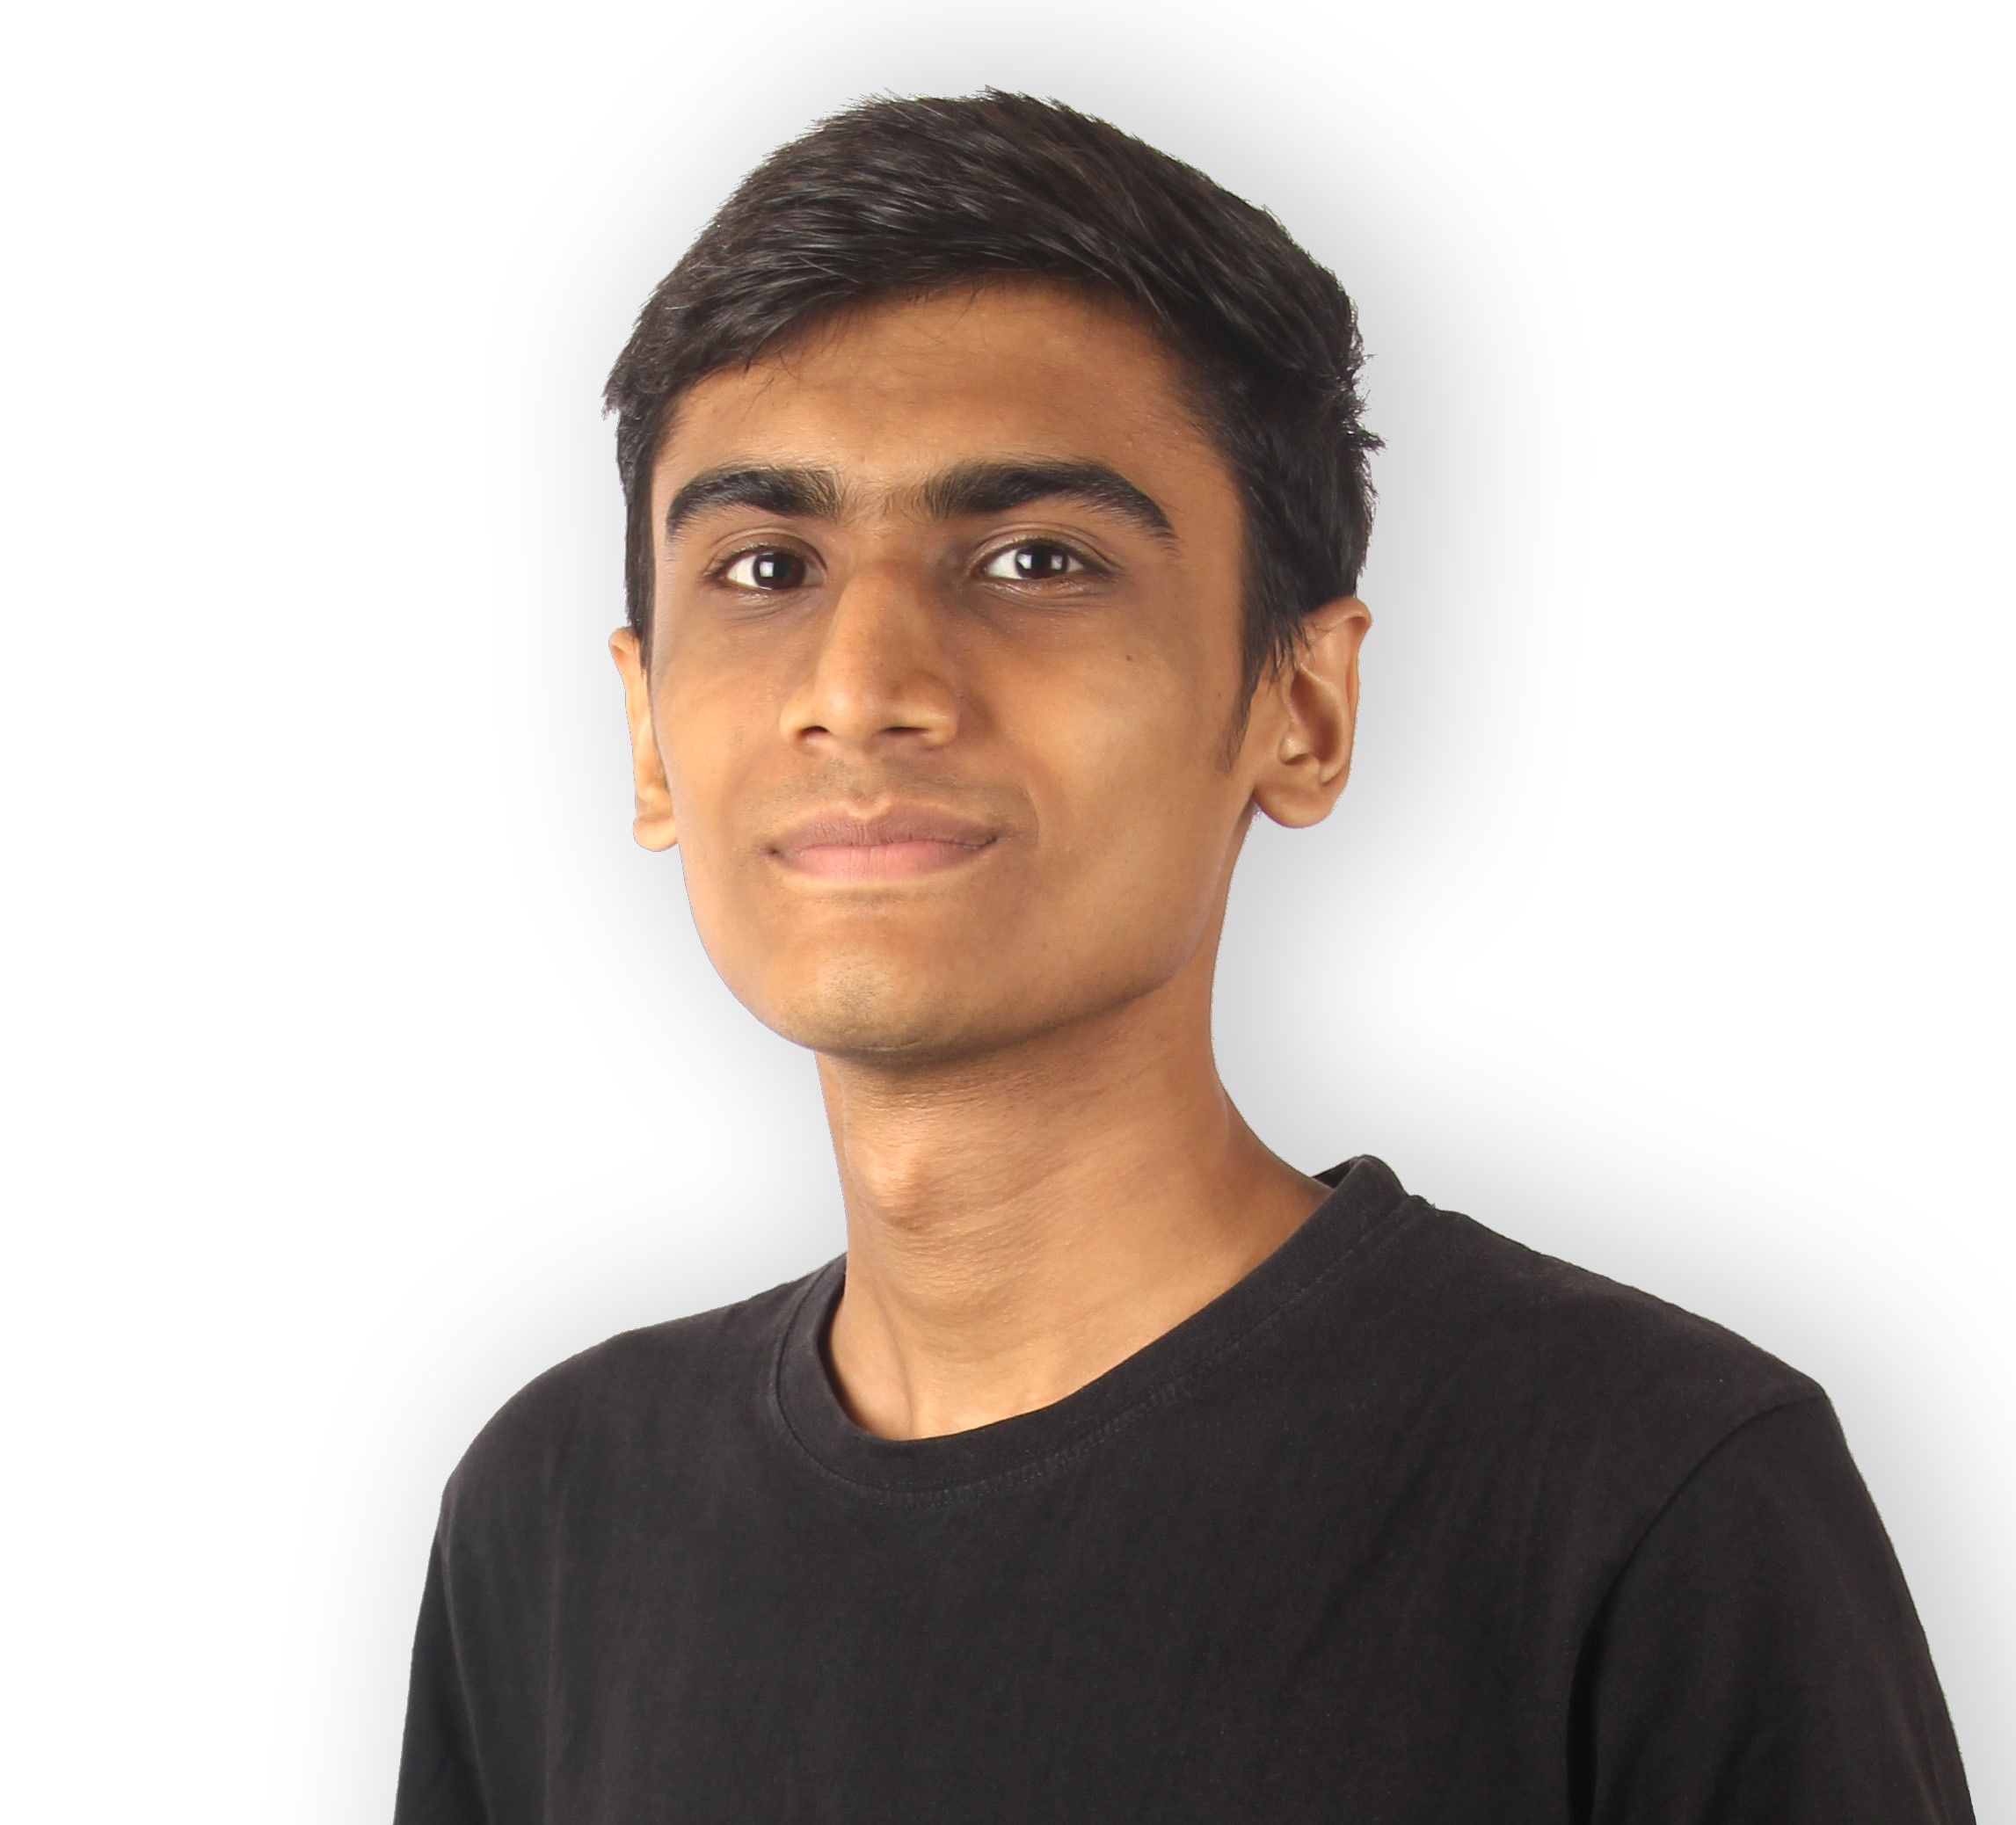
\includegraphics[height=2.5cm]{fig/lec01/Tatsat.jpg}
				\caption*{Tatsat Baldaniya}
		\end{figure}
		\column[T]{0.33\textwidth}
		\begin{figure}
			\centering
				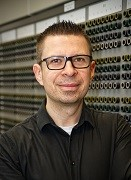
\includegraphics[height=2.5cm]{fig/lec01/pawel.jpg}
				\caption*{Pawel Malicki}
		\end{figure}		
	\end{columns}
	\vspace{-0.5cm}
	\begin{varblock}{Contact}
		\begin{itemize}
			\item Email: see \href{https://www.eti.uni-siegen.de/ias/}{chair's homepage}
			\item Offices: H-A building, 4th floor
			\item Individual appointments on request (remote or personally)
            \item Multiple relevant courses are offered by the Chair.  \href{https://www.eti.uni-siegen.de/ias/teaching/}{Check link!}
		\end{itemize}
	\end{varblock}
%** \small{Future follow-up courses are planned to be introduced in next semester- High Frequency Power Electronics, etc.}
	\end{frame}



%%%%%%%%%%%%%%%%%%%%%%%%%%%%%%%%%%%%%%%%%%%%%%%%%%%%%%%%%%%%%
%% Start %%
%%%%%%%%%%%%%%%%%%%%%%%%%%%%%%%%%%%%%%%%%%%%%%%%%%%%%%%%%%%%%
\begin{frame}
\center
\textbf{\huge{Module I: Introduction to Automation Technologies}}
\end{frame}

%%%%%%%%%%%%%%%%%%%%%%%%%%%%%%%%%%%%%%%%%%%%%%%%%%%%%%%%%%%%%
%% What is Electronics %%
%%%%%%%%%%%%%%%%%%%%%%%%%%%%%%%%%%%%%%%%%%%%%%%%%%%%%%%%%%%%%
% \begin{frame}
% 	\frametitle{What are "Electronic Devices"?}
% 	\begin{columns}
% 		\begin{column}{0.5\textwidth}
% 			\begin{varblock}{Electronic Devices}
% 				Electronic devices are hardware components which leverage the property of materials to control the flow of electrons or charge.
% 			\end{varblock} \vspace{-0.5cm}		
% 			\begin{itemize}
% 				\item<2-> Have a long history of development- started with the invention of vaccum tube or Thermionic valve in 1904 by J.A. Fleming.
% 				\item<3-> The first transistor was invented in 1947 by J.Bardeen, W.H. Brattain and W.S. Shockley in Bell Labs.
% 				\item<4-> The first integrated circuit was invented in 1958 by J. Kilby and R. Noyce -- On and it goes
% %				\item<5-> The first microprocessor was invented in 1971 by F. Faggin, T. Klein and H. Hoff in Intel.
% %				\item<6-> The first microcontroller was invented in 1971 by F. Faggin, T. Klein and H. Hoff in Intel.
% %				\item<7-> On and it goes- every day new devices are invented and developed.
% 			\end{itemize}
% 		\end{column}
% 		\begin{column}{0.5\textwidth}
% 			\begin{figure}
% 				\centering
% 				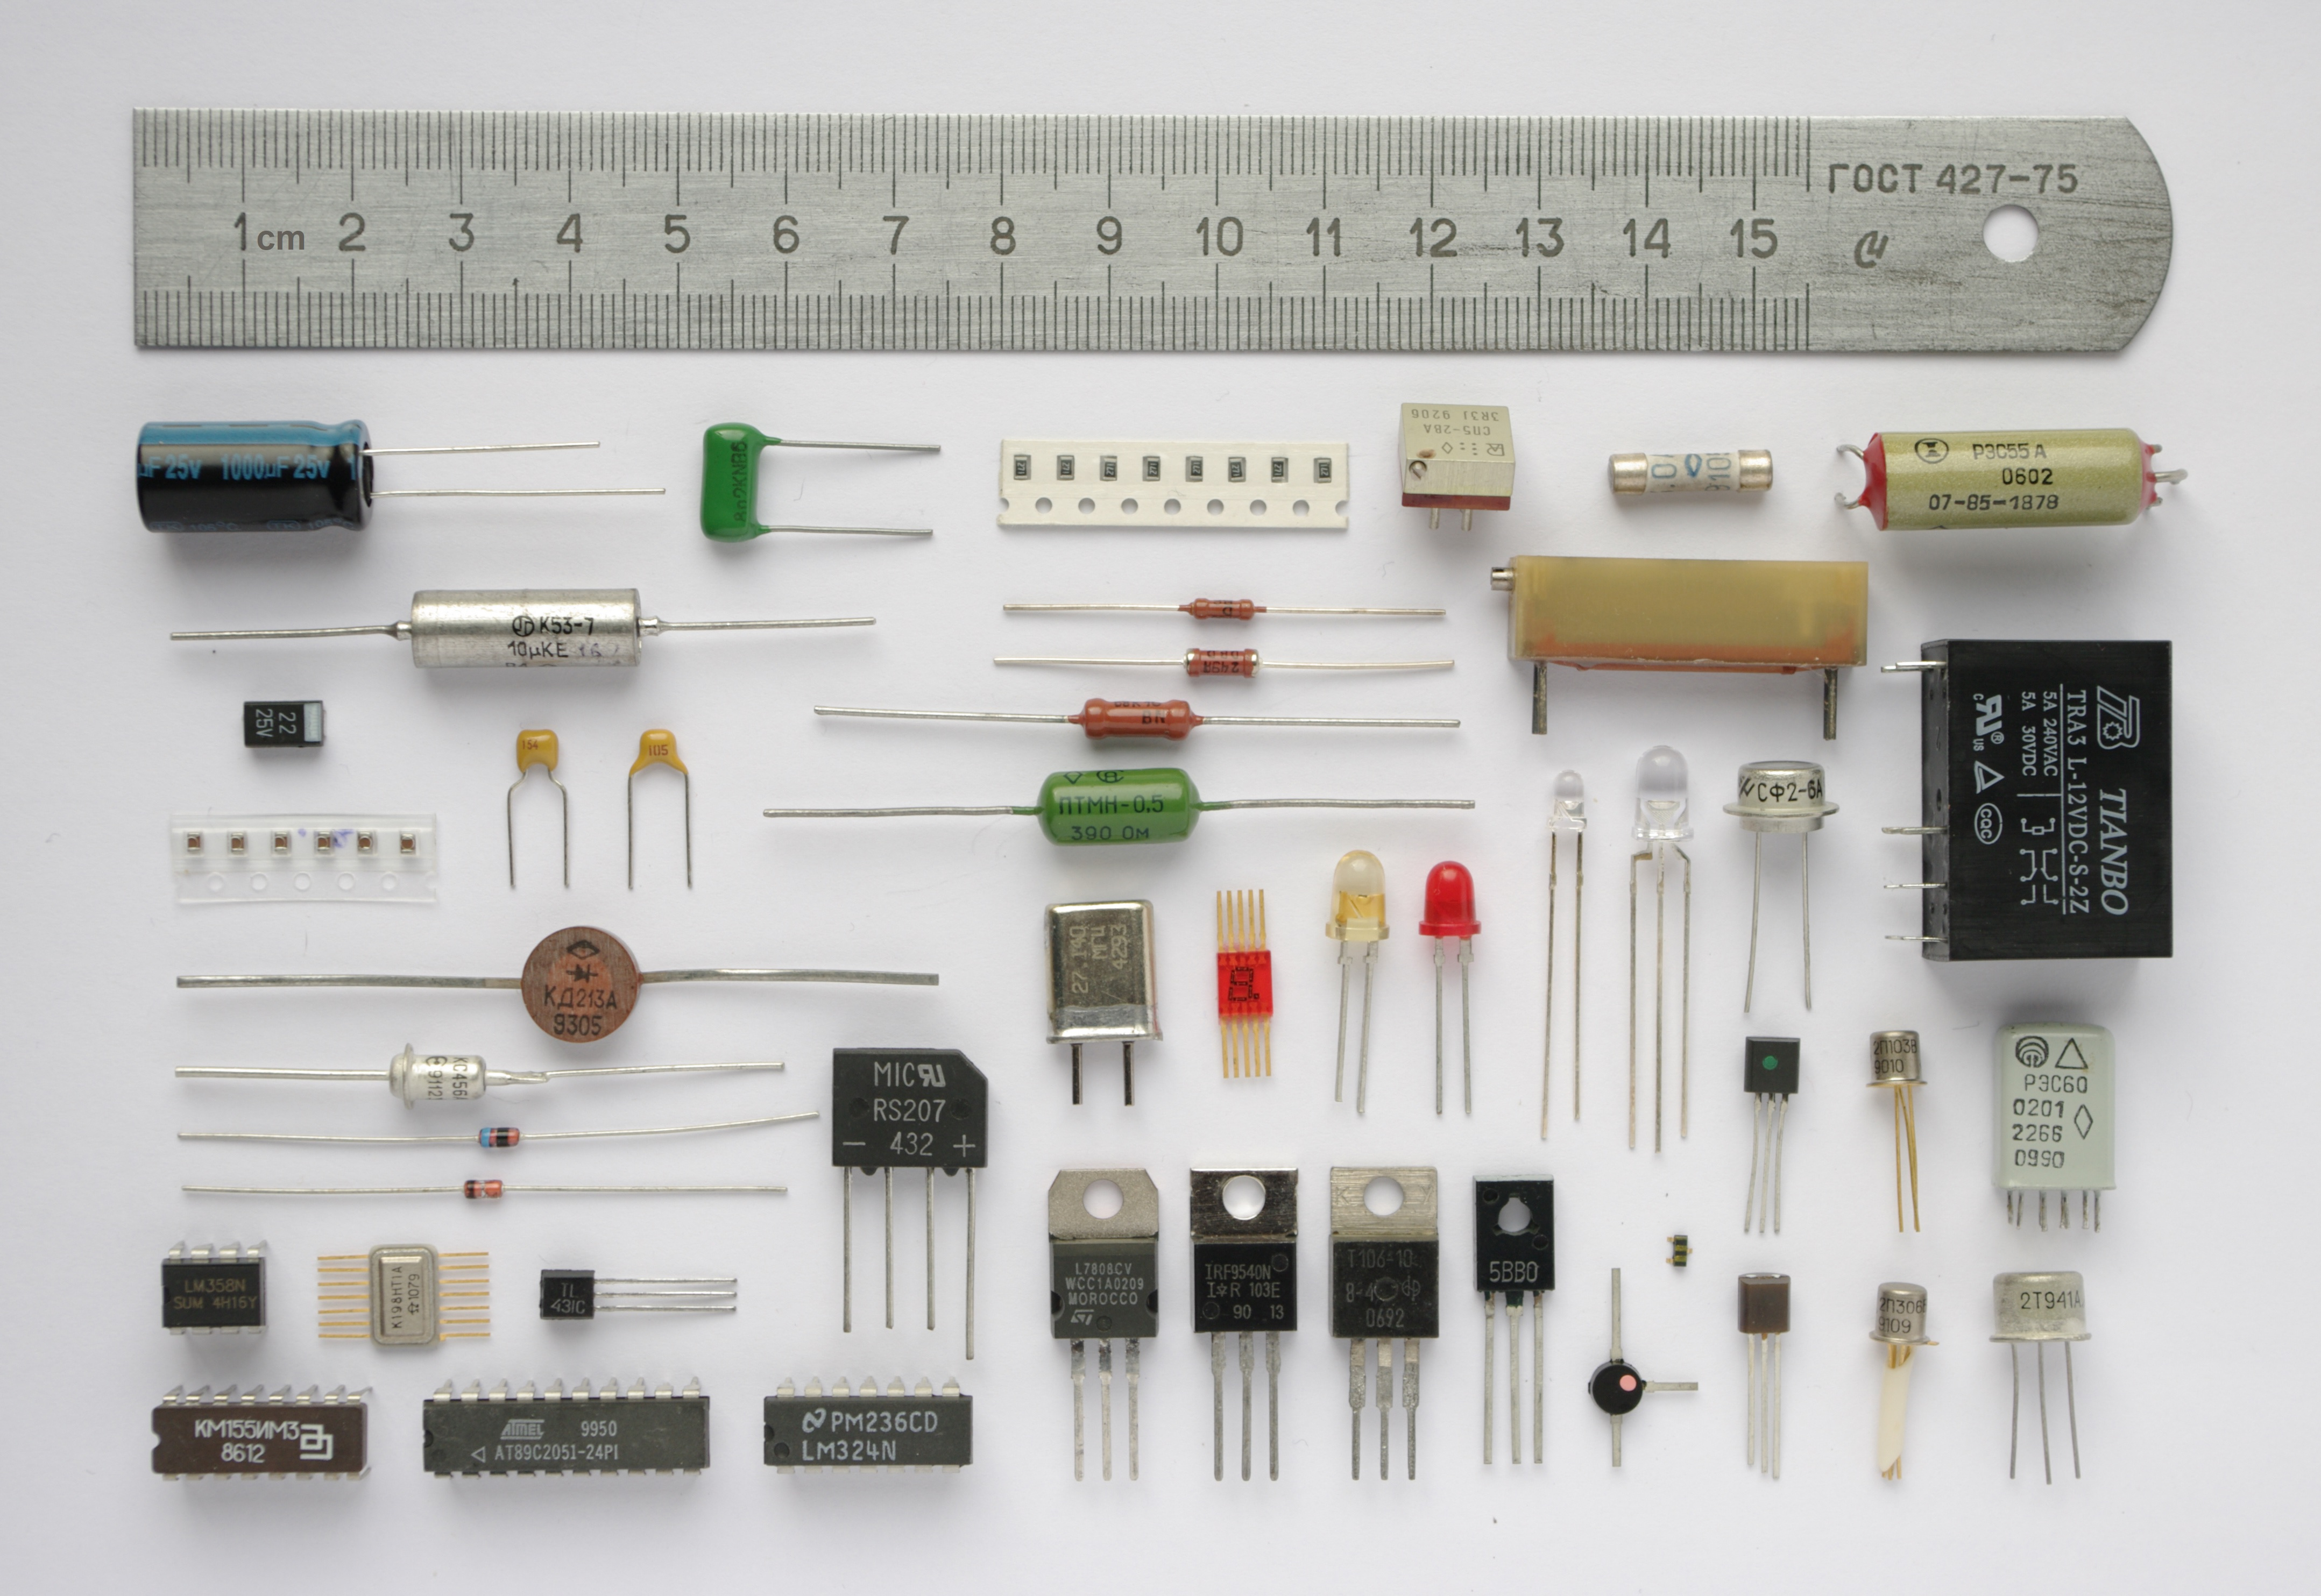
\includegraphics[scale= 0.05]{fig/lec01/Componentes.jpg}
% 				\caption{Example of electronic components (source: \href{https://commons.wikimedia.org/wiki/File:Componentes.JPG}{Wikimedia Commons}, Kae, public domain)}
% 			\end{figure}
% 		\end{column}
% 		\end{columns}
% \end{frame}



% --- Slide 1: What is Automation? ---
\begin{frame}{What is \textit{Automation}?}
\textbf{Working definition for this course}\\[2mm]
\emph{Automation is the purposeful application of mechanical, electrical, and computer technologies to reduce human involvement in task performance—without necessarily removing humans from the loop.}

\vspace{2mm}
\textbf{Key nuances}
\begin{itemize}
  \item \textbf{Displace vs. replace:} automation often reallocates human effort to higher-value tasks rather than eliminating it.
  \item \textbf{Hardware \& software co-design:} improvement may be purely software (e.g., CAD workflows) or mechatronic (robotic cells).
  \item \textbf{Beyond factories:} retail checkout, medical devices, energy systems, mobility—all are automation domains.
\end{itemize}

%\vspace{2mm}
\end{frame}

\begin{frame}{Examples of Automation}
%\textbf{Illustrative examples}
	\begin{columns}
		\begin{column}{0.25\textwidth}
			\begin{itemize}
  				\item \emph{Self-checkout:} barcode + payment automation reduces repetitive cashier tasks while keeping supervision.
			\end{itemize}
		\end{column}
		\begin{column}{0.75\textwidth}
				\begin{figure}
				\centering
				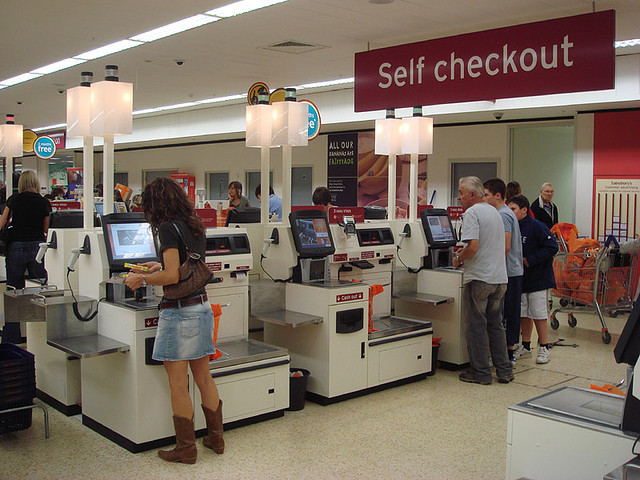
\includegraphics[width=0.7\linewidth]{fig/lec01/Self_checkout.jpg}
				\caption*{Self checkout machines (Source: from \href{https://commons.wikimedia.org/wiki/File:Self_checkout_using_NCR_Fastlane_machines.jpg}{Self checkout using NCR Fastlane machines}, \href{https://creativecommons.org/licenses/by/2.0/deed.en}{CC BY 2.0})}
			\end{figure}
		\end{column}
\end{columns}
\end{frame}

\begin{frame}{Examples of Automation}
%\textbf{Illustrative examples}
	\begin{columns}
		\begin{column}{0.25\textwidth}
			\begin{itemize}
				\item \emph{Computer Aided Design (CAD) evolution:} from manual drafting to 3D solid modeling, numerical control code, and auto-documentation.
			\end{itemize}
		\end{column}
		\begin{column}{0.75\textwidth}
				\begin{figure}
				\centering
				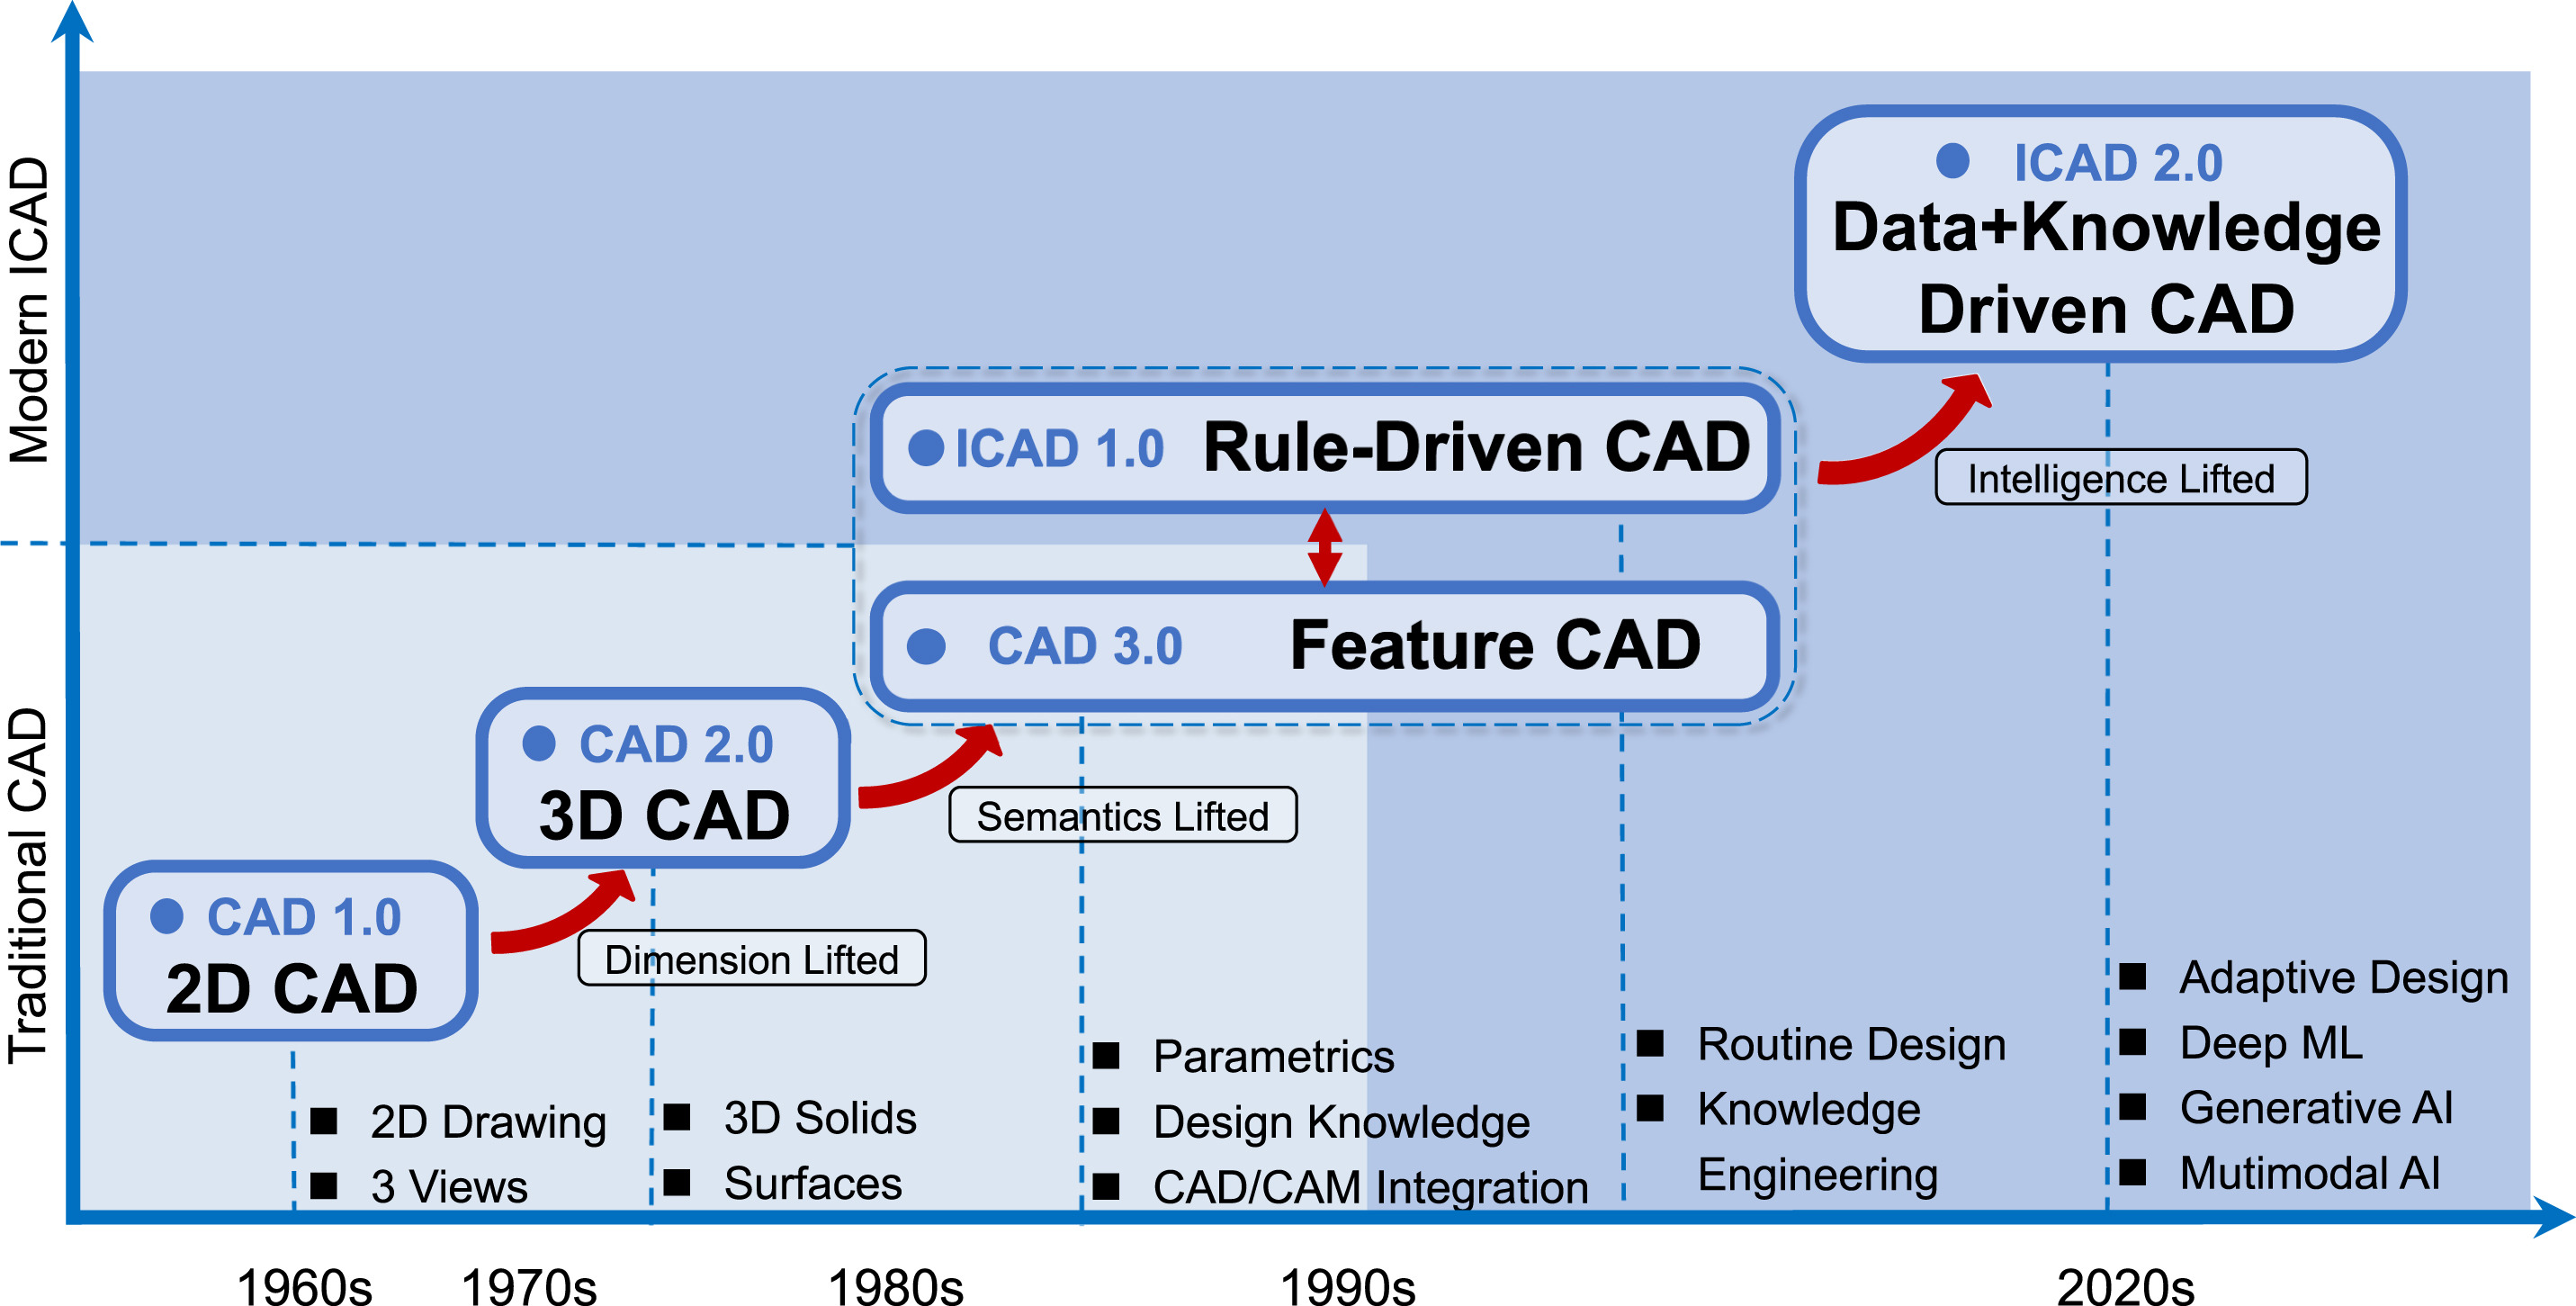
\includegraphics[width=0.8\linewidth]{fig/lec01/CAD_development.jpg}
				\caption*{Historical development of CAD (Source: Zou, Qiang, Yingcai Wu, Zhenyu Liu, Weiwei Xu, and Shuming Gao. "Intelligent CAD 2.0." Visual Informatics 8, no. 4 (2024): 1-12.)}
			\end{figure}
		\end{column}
\end{columns}
\end{frame}




% --- Slide 2: Why Now? Value & Impact ---
\begin{frame}{Why Now? Value, Impact, and Trends}
\textbf{What automation accomplishes today}
\begin{itemize}
  \item Enables \textbf{flexible value networks}: rapid changeovers, mass customization, and supply-chain visibility.
  \item Integrates \textbf{heterogeneous technologies} across disciplines; links physical assets to \textbf{digital representations}.
  \item Improves \textbf{quality, safety, and energy efficiency}; turns data into decisions.
\end{itemize}

\textbf{Where it is going}
\begin{itemize}
  \item From real-time control of single machines to \textbf{orchestration} of whole cells/lines and ecosystems.
  \item \textbf{Autonomous capabilities}: perception, context understanding, and bounded autonomy with human oversight.
  \item \textbf{Sustainability and circularity}: traceability, footprint accounting, and lifecycle optimization.
\end{itemize}
\end{frame}


\begin{frame}{Why Now? Value, Impact, and Trends}
	\begin{columns}
		\begin{column}{0.25\textwidth}
			\textbf{Practical life example}\\
				Battery cycler cell: recipe engine (e.g., CC-CV-rest), interlocks, data historian, remote diagnostics, and energy-aware scheduling.
		\end{column}
		\begin{column}{0.75\textwidth}
				\begin{figure}
				\centering
				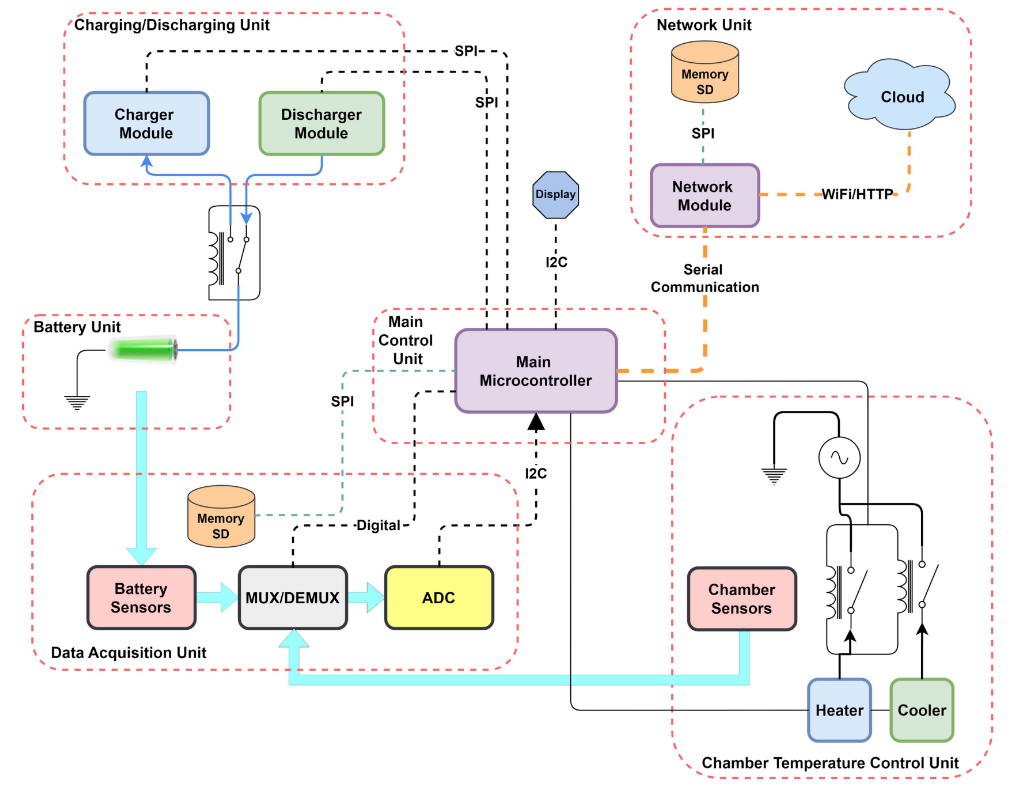
\includegraphics[width=0.7\linewidth]{fig/lec01/cell_test_automation.png}
				\caption*{Automated cell test set-up (Source: \href{https://doi.org/10.1109/TIA.2025.3561705}{Mulpuri et. al.,IEEE Trans. on Industry Appl., vol. 61-5})}
			\end{figure}
		\end{column}
\end{columns}
\end{frame}


\begin{frame}{Nature and Scope of Automation}
\textbf{Automation can occur anywhere humans perform structured tasks.}
\begin{itemize}
  \item Includes entertainment (remote controls), offices (data entry), transportation, and healthcare.
  \item Combines mechanical, electrical, and computer elements-modern systems are hybrid and interlinked.
  \item Machines themselves can contain smaller automated subsystems, leading to hierarchical automation.
\end{itemize}

\vspace{3mm}
\textbf{Essence:}  
Automation evolves continually, driven by technology that reduces human effort, improves precision, and enhances reliability across diverse applications.
\end{frame}

\begin{frame}{Automation Technology Today and Tomorrow}
\textbf{Current accomplishments :} as per the Society for Measurement and Automation Technology within the Association of German Engineers (VDI/VDE) outlook:
\begin{itemize}
  \item Enables \textbf{flexible value networks} and digital connectivity.
  \item Makes technology more accessible and user-friendly.
  \item Integrates mechanical, electrical, and information technologies.
  \item Connects \textbf{real-world physical elements} with their \textbf{digital representations}.
\end{itemize}

\vspace{3mm}
\textbf{Emerging directions}
\begin{itemize}
  \item Intelligent, networked products capable of autonomous action.
  \item Sustainability and circular economy supported by digital transparency.
  \item Need for clear standards, security, and qualified human oversight.
\end{itemize}
\end{frame}

\begin{frame}{Self-Perception of Automation Technology}
\textbf{A multidisciplinary field:}
\begin{itemize}
  \item Integrates \textbf{mechanical, electrical, computer, and information engineering}.
  \item Engineers act as \textbf{system integrators}—coordinating diverse components into a coherent whole.
\end{itemize}

\vspace{3mm}
\textbf{Historical evolution:}
\begin{itemize}
  \item From mechanical aids to networked, software-defined systems.
  \item Increased productivity and flexibility through information technology.
\end{itemize}

\vspace{3mm}
\textbf{Future perspective:}
\begin{itemize}
  \item Toward \textbf{autonomous systems} that perceive, decide, and act.
  \item Humans remain central—for supervision, creativity, and ethical responsibility.
\end{itemize}
\end{frame}




% --- Slide 3: The Automation Stack (Mechatronics Lens) ---
\begin{frame}{The Automation Stack (Mechatronics Lens)}
\begin{columns}[T,onlytextwidth]
\column{0.54\textwidth}
\textbf{Layers}
\begin{enumerate}
  \item \textbf{Sensors} (electrical, mechanical, magnetic, optical) $\rightarrow$ scaling, filtering, calibration, shielding.
  \item \textbf{Compute} (MCU/DSP, FPGA, PLC): timing, determinism, safety tasks, OS/RTOS.
  \item \textbf{Control \& Sequencing}: PID/IMC, cascades, feedforward; SFC/state machines, interlocks, mode logic.
  \item \textbf{Actuators \& Drives}: DC/BLDC/servo, VFD/FOC, motion profiles, STO.
  \item \textbf{Comms \& Data}: OPC~UA, Modbus‐TCP, MQTT; time sync, historians, dashboards.
  \item \textbf{Supervision \& Optimization}: HMI/SCADA, digital twins, KPIs (OEE), diagnostics, updates.
\end{enumerate}

\column{0.44\textwidth}
\centering
%\includegraphics[width=\linewidth]{stack_placeholder.png}\\[-1mm]
\footnotesize{Block diagram placeholder: Sensor $\to$ Conditioning $\to$ Compute $\to$ Actuator, with data to SCADA/Cloud.}
\end{columns}

\vspace{1mm}
\textbf{System integrator view} \\
Automation engineers orchestrate multiple “couples” (machines/cells) to dance in unison: coordination, timing, safety, and lifecycle management.
\end{frame}


%%%%%%%%%%%%%%%%%%%%%%%%%%%%%%%%%%%%%%%%%%%%%%%%%%%%%%%%%%%%%
%% Necessary prior knowledge %%
%%%%%%%%%%%%%%%%%%%%%%%%%%%%%%%%%%%%%%%%%%%%%%%%%%%%%%%%%%%%%
\begin{frame}
	\frametitle{Necessary prior knowledge for this course}
	You should have a basic understanding of the following topics:
	\begin{itemize}
		\item Basic electrical engineering knowledge (e.g., Ohm's law, Kirchhoff's laws, etc.)
		\item Basic understanding of physics in electronics
		\item Algebra and complex numbers
		\item Basic signal theory knowledge (e.g., Fourier series, Laplace transform)
		\item No advanced knowledge of semiconductors or programming is needed — this course builds those concepts from scratch and applies them to real systems.
	\end{itemize}
	\vspace{0.5cm}
	\onslide<2->What we will \underline{not} cover, but you do not need to know (covered in separate courses):
	\begin{itemize}
		\item Power converter circuits and topologies.
		\item Power electronics in depth involving analysis and controller design. 
	\end{itemize}
\end{frame}

%%%%%%%%%%%%%%%%%%%%%%%%%%%%%%%%%%%%%%%%%%%%%%%%%%%%%%%%%%%%%
%% Recommended reading %%
%%%%%%%%%%%%%%%%%%%%%%%%%%%%%%%%%%%%%%%%%%%%%%%%%%%%%%%%%%%%%
\begin{frame}
	\frametitle{Recommended reading}
	\begin{itemize}
		\item Baliga, B. Jayant. Fundamentals of power semiconductor devices. Springer Science \& Business Media, 2010.
		\item Lutz, Josef, Heinrich Schlangenotto, Uwe Scheuermann, and Rik De Doncker. "Semiconductor power devices." Physics, characteristics, reliability 2 (2011).
		\item Baliga, B. Jayant, ed. Wide Bandgap Semiconductor Power Devices: Materials, Physics, Design, and Applications. Woodhead Publishing, 2018.
		\item K. Niayesh, M. Runde, "Power Switching Components Theory, Applications and Future Trends", 1. Ed., Springer, 2018.
	\end{itemize}
\end{frame}